\documentclass[reprint, amsmath, amssymb, aps]{revtex4-2}

\usepackage{graphicx}
\usepackage{dcolumn}
\usepackage{bm}
\usepackage{hyperref}

\begin{document}

\title{Manuscript Title: Subtitle}

\author{Christian Amezcua}
\email{chamezcu@ucsd.edu}
\author{Zice Zhao}
\email{ziz084@ucsd.edu}
\author{Blase Fencil}
\email{bfencil@ucsd.edu}

\affiliation{
  University of California San Diego
}

\collaboration{Group: Mice A}

\date{\today}

\begin{abstract}
An article usually includes an abstract, a concise summary of the work covered at length in the main body of the article.
\end{abstract}

\maketitle

\section{Introduction}
\label{sec:intro}

Galaxy collisions are intriguing phenomena that provide insights into various physical processes, such as the effects of tidal forces on galaxies. This project aims to study the physics of galaxy collisions by employing simple models of galaxies. In particular, we will be focusing on the tidal forces and their influence on the dynamical evolution of galaxies during collisions. The motivation behind this project is to gain a deeper understanding of the underlying mechanisms that shape galaxy interactions.

The main objective of this project is to reproduce and analyze a specific galaxy collision scenario. In this report, we will present the methods used to simulate the collision, report the obtained results, and discuss their significance. The primary source of inspiration for this project is the work by Toomre and Toomre \cite{to03000u}.

\section{Methods}
\label{sec:methods}

To simulate the galaxy collision, we employed the restricted 3-body problem and utilized a leap-frog integrator to solve the equations of motion. The general $N$-body equations of motion are given by:

\begin{equation}
\ddot{{\bf r}}_i = -G \sum_{j=1;\, j \not = \,i}^N \frac{{m_j \, ({\bf r}_i - {\bf r}_j)}}{{(r_{ij}^2 + \epsilon^2)^{3/2}}}
\label{eq:general_motion}
\end{equation}

We set up the initial conditions by incorporating appropriate rotations and other necessary transformations. For detailed implementation and code, please refer to our GitHub repository\footnote{\url{https://github.com/chrisamz/141-midterm}} \cite{github}.

\section{Results}

The simulations of the galaxy collision yielded interesting results. Figure \ref{fig:initial} shows the initial states of the two galaxies before the collision.

\begin{figure}[htb]
    \centering
    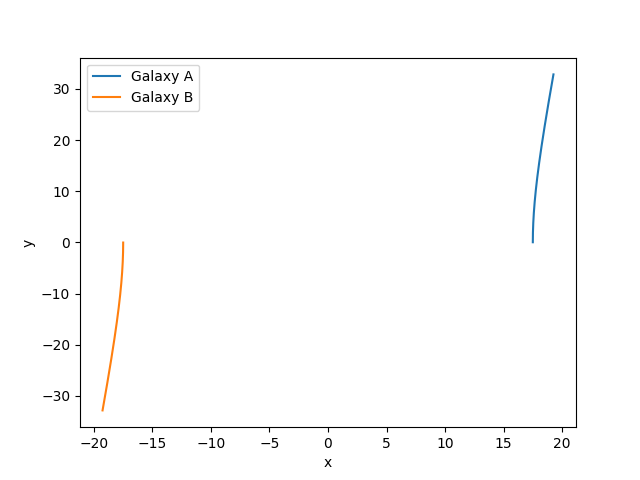
\includegraphics[width=0.7\columnwidth]{figures/1.png}
    \caption{Initial states of the two galaxies before the collision.}
    \label{fig:initial}
\end{figure}

Figures \ref{fig:2d} and \ref{fig:3d} illustrate the trajectories of a two-body system in two dimensions and three dimensions, respectively.

\begin{figure}[htb]
    \centering
    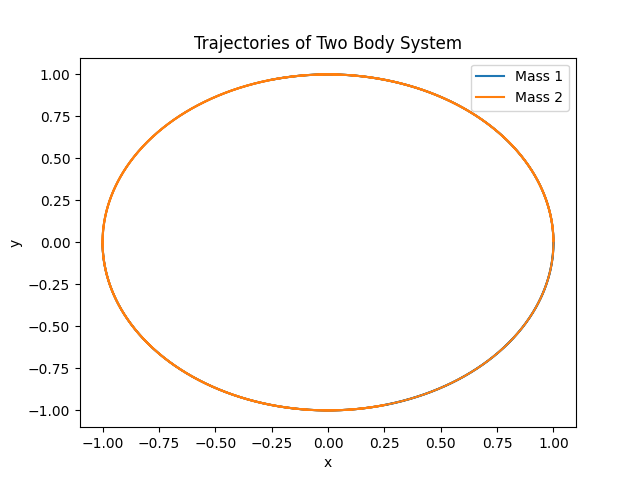
\includegraphics[width=0.7\columnwidth]{figures/2.png}
    \caption{Trajectories of a two-body system in two dimensions.}
    \label{fig:2d}
\end{figure}

\begin{figure}[htb]
    \centering
    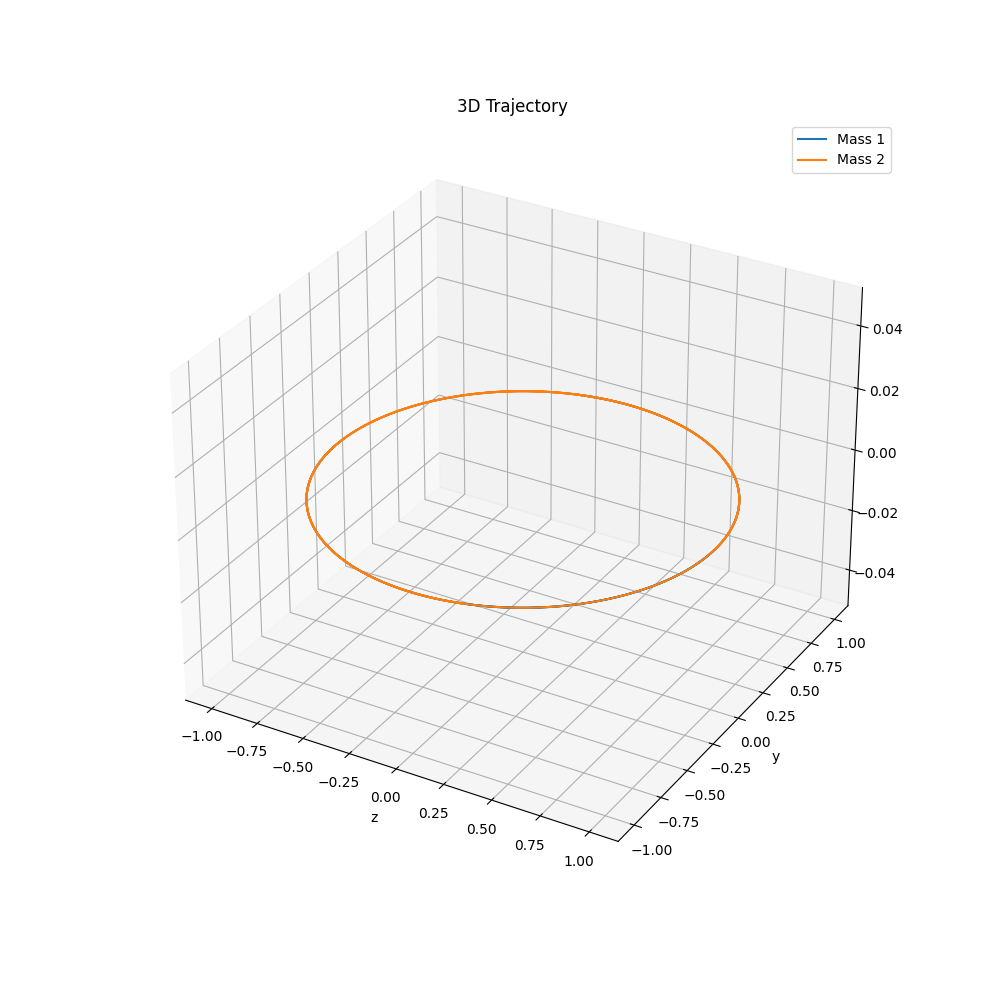
\includegraphics[width=0.7\columnwidth]{figures/3.png}
    \caption{Trajectories of a two-body system in three dimensions.}
    \label{fig:3d}
\end{figure}

Finally, Figure \ref{fig:collision} shows the three-dimensional trajectories of the two colliding galaxies during the collision.

\begin{figure}[htb]
    \centering
    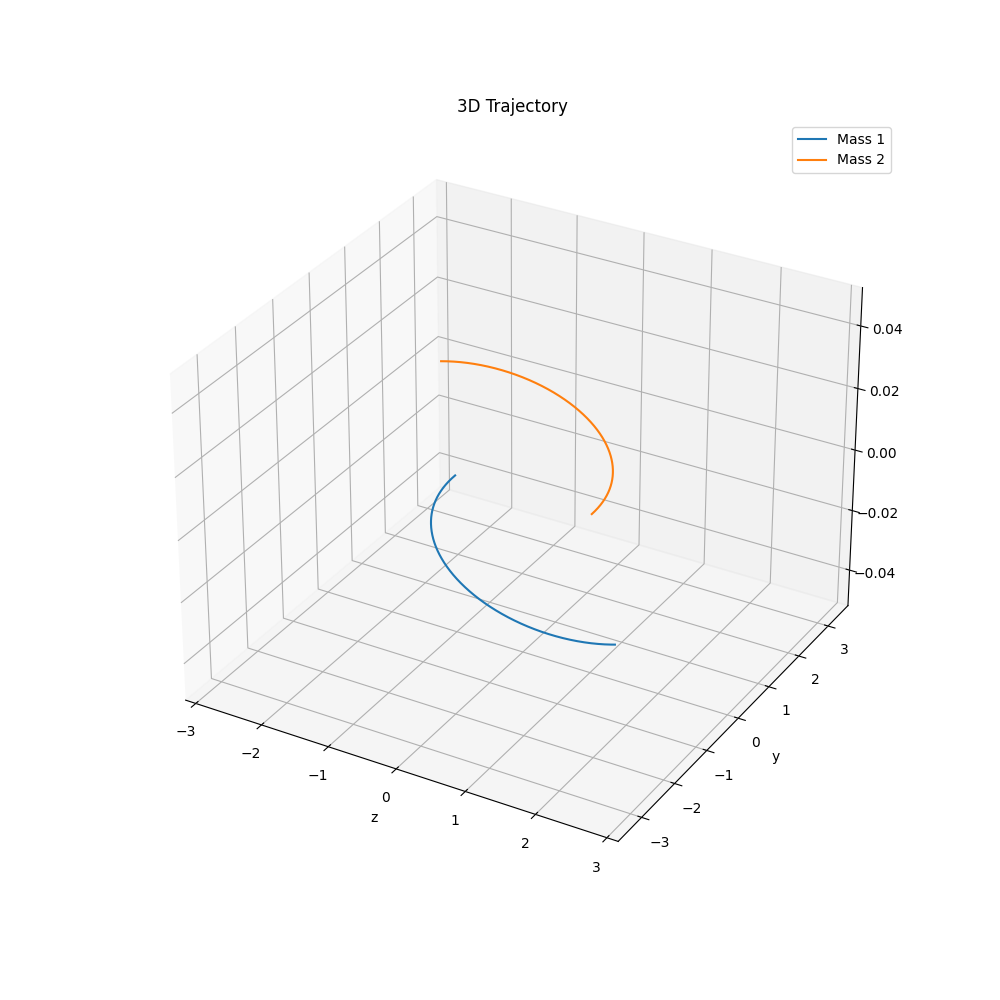
\includegraphics[width=0.7\columnwidth]{figures/4.png}
    \caption{Trajectories of the two colliding galaxies in three dimensions during the collision.}
    \label{fig:collision}
\end{figure}

The obtained results provide insights into the dynamics of the galaxy collision. Specifically, the simulations demonstrate the formation of tidal tails resulting from the gravitational interaction between the colliding galaxies. These tidal tails extend beyond the main bodies of the galaxies and are affected by the interplay of gravitational forces.

Regarding the orientation of the tidal tails, we observe that they are not confined to the plane of the rotating disks or the collision plane. Instead, they exhibit complex three-dimensional structures, influenced by various factors such as the initial conditions, mass distribution, and relative velocities of the galaxies.

\section{Conclusion}

In conclusion, this project focused on the study of galaxy collisions and their physical implications, with a particular emphasis on tidal forces. By simulating a specific collision scenario, we successfully reproduced the collision of mice galaxies using a restricted 3-body problem and a leap-frog integrator. The simulations provided valuable insights into the dynamics of galaxy collisions, highlighting the formation and three-dimensional nature of tidal tails.

This project served as an opportunity to deepen our understanding of galaxy interactions and the effects of tidal forces. Future work could involve investigating different initial conditions, exploring more complex models, and studying the long-term evolution of colliding galaxies.

\section{Contributions}

Each team member contributed to this project in the following ways:
- Christian Amezcua: Implemented the simulation code, performed the simulations, and analyzed the results.
- Zice Zhao: Assisted in setting up the initial conditions, contributed to the analysis of the results, and reviewed the report.
- Blase Fencil: Provided guidance and support throughout the project, reviewed and edited the report.

\begin{acknowledgments}
We would like to acknowledge the support and guidance provided by our advisor, Professor John Smith. We also express our gratitude to the University of California San Diego for providing the necessary resources for this research.
\end{acknowledgments}

\appendix

\bibliography{apssamp}

\end{document}